\chapter{Cyclic polytopes}

\scribe{Anna Somoza}
 
\begin{remark}
We say that a real algebraic curve $t \mapsto (\varphi_1(t), \dots, \varphi_d(t))\in \RR^d$ has degree $d$ if no $d+1$ points on $C$ lie on a hyperplane.
\end{remark}

\begin{theorem}
The convex hull of $n\geq d+1$ points on an algebraic curve of degree $d$ is called the \emph{cyclic polytope} $C_d(n)$, which is a simplicial polytope.
\end{theorem}

Note that we are talking about \emph{the} cyclic polytope, denoting unicity. This is in terms of equivalence between polytopes, a topic that we will now go through.

\section{Notions of equivalence between polytopes $P, Q\subset \RR^d$.}

When we talk about $P$ and $Q$ being equivalent polytopes we usually refer to the existence of some kind of application $T:\RR^d \to \RR^d$ that takes $P$ to $Q$. In this sense, there are different kinds of equivalence:

\begin{itemize}
\item Congruent: $\exists T\in \operatorname{SO}_d(\RR), t\in\RR^d$ such that $TP + t = Q$;
\item Linearly equivalent or isomorphic: is the case when $T\in \operatorname{GL}_d(\RR)$ and $TP = Q$.
\item Affine equivalent or isomorphic: for $T\in\operatorname{GL}_d(\RR), t\in\RR^d$ and $TP + t = Q$.
\item Projectively equivalent or isomorphic: if there exists an admissible projective transformation $T$ that sends $P$ to $Q$. We need that $T^{-1}(H_\infty) \cap P = \emptyset$\footnote{We need this condition because some projective spaces are non orientable, so what we want to keep infinity away from our polytope}.
\item Combinatorially equivalent or isomorphic: this equivalence refers to its structure, \break $\mathcal{F}(P) \cong \mathcal{F}(Q)$, so that the face lattice are equivalent as graded posets.
\end{itemize}

In the case of cyclic polytopes we are in the situation that the convex hull of $d+1$ points are always combinatorially equivalent.

Then we can reformulate the theorem as follows:

\begin{theorem}
The convex hull of $n\geq d+1$ points on an algebraic curve of degree $d$ is called the \emph{cyclic polytope} $C_d(n)$ (up to combinatorial equivalence). The cyclic polytope is a simplicial polytope.
\end{theorem}

\section{How many $k$-dimensional faces does $C_d(n)$ have?}

Every $k$-face of a cyclic polytope can be defined as the intersection of $d-k$ facets. We have to take into account that every facet is defined by a set of $d$ points with the consideration that they have to come in $\lfloor \frac{d}{2} \rfloor$ adjacent pairs so that the hyperplane that they define keep the remaining $n-d$ points at the same side of it.

Then, we claim that $f_k(C_d(n)) = \binom{n}{k}$ if $k\leq \frac{d}{2}$, because once we fix $k$ points we can complete the set of points with adjacent pairs to find a facet containing all, and by this procedure we can find $d-k$ facets so that our $k$ face is defined by the intersection of the found facets.

For the $k > \frac{d}{2}$ see Lecture \ref{lecture4}.

\subsection{How many $n$-gons exist in $\RR^2$?}

Consider the 4-gon consisting on the square of side 1, $\square ^2$.

\begin{figure}[h]
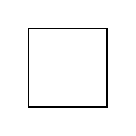
\begin{tikzpicture}
\draw (0,0) -- (1,0) -- (1,1) -- (0,1) -- cycle;
\end{tikzpicture}
\caption{Square of side 1.}
\end{figure}


Then,
%%Here go the example with drawings
\begin{center}

\begin{tabular}{m{4.5cm}m{3cm}m{6cm}}
It is congruent to &
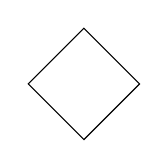
\begin{tikzpicture}
\draw (0,0) -- ({sqrt(2)/2},{sqrt(2)/2}) -- (0,{sqrt(2)}) -- (-{sqrt(2)/2},{sqrt(2)/2}) -- cycle;
\end{tikzpicture}&because it includes rotations,\\
It is affinely equivalent to &
\begin{tikzpicture}
\draw (0,0) -- (2,0) -- (2,2) -- (0,2) -- cycle;
\end{tikzpicture}& because it includes homotecies.\\
It is linearly equivalent to &
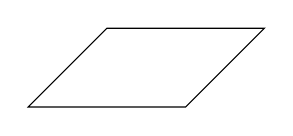
\begin{tikzpicture}
\draw (0,0) -- (2,0) -- (3,1) -- (1,1) -- cycle;
\end{tikzpicture}&because it accepts transformations in the basis.\\
It is projectively equivalent to &
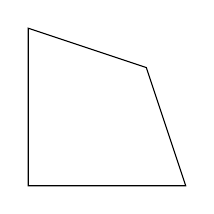
\begin{tikzpicture}
\draw (0,0) -- (2,0) -- (1.5,1.5) -- (0,2) -- cycle;
\end{tikzpicture}&because to define a projection you must fix $d+2$ points.\\
\end{tabular}

\end{center}
\begin{definition}
The \emph{realization space} of a convex polytope $P\subset \RR^d$ with $n$ vertices is $$R(P) = \{ M\in \mathcal{M}_{n\times d}(\RR) \mid P \text{ is projectively equivalent to } \operatorname{conv}\{ \operatorname{col} A\}\}.$$
\end{definition}

%%Include here the image of the Realization space for a 5-gon


\begin{figure}[h]

\begin{tikzpicture}
\definecolor{light-gray}{gray}{0.8}
\path[fill = light-gray] (2,0) -- (7,0) -- (7,2) -- (2,2) -- cycle;
\draw (2,0) -- (0,0) -- (0,2) -- (2,2);
\draw[dashed] (2,2) -- (2,0);
\draw[dashed] (2,2) -- (7,2);
\draw[dashed] (2,0) -- (7,0);
\end{tikzpicture}
\caption{The realization space $R(5-\operatorname{gon})$ so that it is convex.}
\end{figure}

\chapter*{Polytopality of a graph}

The \emph{graph} of a polytope is its 1-skeleton:
$$\operatorname{sk}^k(P) = \{F \leq P \mid \dim(F) \leq k\},$$
$$G(P) = \operatorname{sk}^1(P) = \{\text{vertices and edges in } P\}.$$

We may wonder, given a graph, if it can be the graph for any polytope. That is what we call the polytopality range:

\begin{definition}[Polytopality range]
Let $G$ be a graph. Then, its polytopality range is
$$\operatorname{PR}(G) = \{ d\in \NN \mid \exists P^d \text{ with } \operatorname{sk}^1(P) = G\}$$
\end{definition}

To decide for a certain graph whether it is the graph for a $d$-polytope or not, we can use the following criteria among others:

\begin{theorem}[Steinitz]
$G$ is the graph of a 3-dimensional polytope if and only if it is simple, planar and 3-connected.
\end{theorem}

\begin{theorem}[Balinski]
The graph $G(P)$ is $d$-connected for every $d$-polytope $P$.
\end{theorem}

\begin{definition}
A \emph{principal subdivision} of a graph $G$ is a subdivision of the edges of $G$ into paths, such that there exist a so-called principal vertex with the property that edges incident to it are not subdivided.
\end{definition}

\begin{proposition}[$d$-PSP property]
Let $P$ be a $d$-polytope. Then, every vertex in $G(P)$ is the principal vertex of a principal subdivision $K_{d+1}$.
\end{proposition}

\begin{figure}[h!]
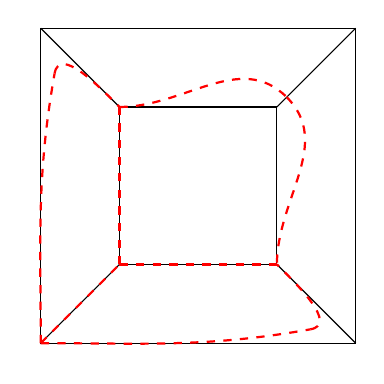
\begin{tikzpicture}
\draw (3.3,0.3) node (A) {};
\draw (0.3,3.3) node (B) {};
\draw (3,3) node (C) {};
\draw (0,0) -- (4,0) -- (4,4) -- (0,4) -- cycle;
\draw (1,1) -- (1,3) -- (3,3) -- (3,1) -- cycle;
\draw (0,0) -- (1,1);
\draw (4,0) -- (3,1);
\draw (0,4) -- (1,3);
\draw (4,4) -- (3,3);
\draw[thick, dashed, red] (0,0) edge[out=0, in=-170] (A.south east);
\draw[thick, dashed, red] (A.south east) edge[out=10, in=-45] (3,1);
\draw[thick, dashed, red] (0,0) -- (1,1);
\draw[thick, dashed, red] (1,1) -- (3,1);
\draw[thick, dashed, red] (1,1) -- (1,3);
\draw[thick, dashed, red] (0,0) edge[out=90, in=-100] (B.north west);
\draw[thick, dashed, red] (B.north west) edge[out=80, in=135] (1,3);
\draw[thick, dashed, red] (1,3) edge[out=0, in=135] (C.north east);
\draw[thick, dashed, red] (C.north east) edge[out=-45, in=90] (3,1);
\draw (0,0) node[circle,  red] {};
\draw (1,1) node[red] {};
\draw (1,3) node[red] {};
\draw (3,1) node[red] {};
\end{tikzpicture}
\caption{This graph has the $3$-PSP property because we have fount a $K_4$ minor.}
\end{figure}

\begin{corollary}
No graph of a 3-polytope is the graph of a $d$-polytope with $d\geq 4$. Therefore, graphs of $3$-polytopes are dimensionally unambiguous, i.e. if it is a 3-polytope graph its polytopality range is $\{3\}$.
\end{corollary}

We get this corollary as a consequence of the $d$-PSP property, because if there was $d^*\geq 4$ such that it was a $d^*$-polytope, it would contain a principal subdivision of $K_{d^* +1}$, $d^* + 1 \geq 5$, so it would in particular contain a $K_5$-minor.
% Local Variables: 
% mode: pdflatex
% TeX-master: "dag-upc"
% End: 
